\documentclass[a4paper,11pt]{article}
\usepackage[osf]{mathpazo}
\usepackage{ms}
\usepackage[sort&compress]{natbib}
\raggedright

\newcommand{\plant}{\textsc{plant}}

\usepackage[colorinlistoftodos]{todonotes}

\title{{\plant}: A package for modelling forest trait ecology \& evolution}
\author{Daniel S. Falster, Richard G. FitzJohn, and Mark Westoby}
\affiliation{
Department of Biological Sciences, Macquarie University, Sydney, NSW 2109, Australia\\
Email for correspondence: \texttt{daniel.falster@mq.edu.au}\\
A manuscript in consideration as a research paper for
publication in MEE as part of the Special Feature \emph{Demography
  beyond the Population}.}
\date{}

\bibliographystyle{mee}

\usepackage[title,titletoc,toc]{appendix}

\mstype{Applications Note}
\runninghead{plant}
\keywords{demography, emergent, fitness, growth,
physiology, metapopulation, mortality, reproduction, size-structure,
tradeoff}

\begin{document}
\mstitlepage
\noindent
\parindent=1.5em
\addtolength{\parskip}{.3em}
\doublespacing
\linenumbers
\section{Summary}\label{abstract}
\begin{enumerate}
\def\labelenumi{\arabic{enumi}.}
\itemsep1pt\parskip0pt\parsep0pt
\item
  Population dynamics in forests are strongly size-structured:
  larger plants shade smaller plants while also expending
  proportionately more energy on building and maintaining woody stems.
  Although the importance of size-
  structure for demography is widely recognised, many mechanistic models
  either omit it entirely, or include only coarse approximations.
\item
  Here we introduce the {\plant} package (TRait Ecology and Evolution), an
  extensible framework for modelling plant demography across the entire
  life cycle and in structured metapopulations, via coupled differential equations.
  At its core, {\plant} is an
  individual-based mechanistic model where plant physiology and demography is mediated by
  traits. Individuals from multiple species can be grown in isolation,
  in patches of competing plants, or in metapopulations under a
  disturbance regime. Dynamics within patches of competing plants are
  resolved using novel extensions of the ``Escalator Boxcar Train''
  technique. Combined effects of trait-, size- and patch-structured
  dynamics are integrated into population level estimates of
  reproductive fitness.
\item
  {\plant} is an open source R package and is available at
  \href{https://github.com/traitecoevo/plant}{github.com/traitecoevo/plant}.
  While accessed from R, the core routines in {\plant} are written in C++.
  The package provides for alternative physiologies and for
  hyper-parameterisation to capture trade-offs among parameters. A
  detailed test suite is provided to ensure correct behaviour of the code.
\item
  We provide worked examples illustrating {\plant}'s use to study the
  influence of functional traits on growth of individual plants, of
  whole patches and on assembly of ecological communities.
\end{enumerate}

\section{Introduction}\label{introduction}

Plant growth and demography are fundamentally size- and trait-
structured, influencing dynamics over time-scales ranging from
instantaneous physiological effects to long-term evolutionary outcomes
\citep{Harper-1977, Westoby-2002}. As an individual increases its leaf
area, it increases its potential to generate photosynthate.  In
contrast, as indivuduals grow, they must use increasing fractions of
this photosynthetic income to building and maintaining support tissues
rather than to new leaves \citep{Givnish-1988, Enquist-2007} and
reproduction \citep{Thomas-2011}. Consequently rates of growth and
mortality change with individual size \citep{Muller-2006, Thomas-2011,
  Ruger-2011, Wright-2010}.
%
The patterns of changing growth rate vary by plant traits; leaf
construction costs and wood density affect growth rates and rates of
tissue replacement \citep{Wright-2010}, while seed size and height at
maturation determine start and end points of ontogenetic trajectories
\citep{Westoby-2002}
%
Strong feedbacks emerge between individuals within a forest due to
competition for light and other resources, such that the growth rate
of one individual depends on the size and traits of nearby
individuals.  This makes it difficult to predict demographic processes
without modelling both individual growth and the interactions between
individuals.
% TODO[RGF]: link back things about natural selection, successional
% dynamics, self thinning, trait evolution and species coexistance.

% NOTE[RGF]: I thought this was way overrefrenced and so just kept a
% few oldies.  Please re-add any key ones that you want to see here.
Although the importance of size-structure for vegetation function and
demography has been long been recognised
\citep[e.g.,][]{Harper-1977, Shugart-1980, Hara-1984},
most large-scale mechanistic models of plant growth either omit it
entirely, or only include coarse approximations
\citep{Cramer-2001, Dekauwe-2014, Kelley-2013, Sitch-2003}. The likely
reason is the computational
challenge of modelling size-structured dynamics. 
% TODO[RGF]: I don't see the link with the above?  Can this be
% shortened/tightened?  It's too long for a 3k word paper
During the 1980s and
early 1990s, size-structured ``gap'' models were widely used
\citep[e.g.][]{Huston-1987, Shugart-1980}. These gap models were
parameterised in terms of growth using statistical functions; this meant 
that data had to be collected for each species, limiting widespread application. 
The next generation of models focussed on establishing core physiology for 
a limited number of functional types, and
sacrificed details of demography in order to achieve global coverage
\citep{Haxeltine-1996,Woodward-1995}. This history has brought us to the
current situation where all but a couple
\citep[e.g.][]{Moorcroft-2001, Smith-2014} of the most popular vegetation
models lack size-structure. Instead, most models
are focused on modelling fluxes carbon and water, but say little about
demographic behaviour, and consequently are also unable to account for
any non-linear demographic feedbacks that may arise.

Similarly, most models used in theoretical ecology to explore
questions about species coexistence also lack size-structured dynamics
\citep[e.g.][]{Calcagno-2006, Geritz-1995, Leimar-2013,
  Levin-1974,MacArthur-1967,Tilman-1985}.  It is common to assume
competitive interactions are influenced by size-related traits such as
adult size and seed size, but detailed size-structured demography is
rarely considered, at least for plant models \cite[for animal
examples, see][]{Deroos-1988, Deroos-1992}. Consequently, it has been
difficult to connect mechanisms described in these simplistic models
with type of data often collected in the field, such as physiological
leaf traits, and demographic data on growth and mortality in long-term
monitoring plots \citep{Adler-2013}.

In this note, we introduce the {\plant} package for R \citep{R-2015};
a mechanistic framework for studying the effects of size structure and
trait variation on the demography of individual plants, of patches of
competing plants, and of meta-populations structured by a prevailing
disturbance regime.
%
The {\plant} package builds on much existing work investigating the
effect of traits on vegetation properties and the mechanisms
facilitating coexistence of trait mixtures
\citep{Kohyama-1993,Deroos-1997,Moorcroft-2001,Falster-2011,Falster-2015}.

% TODO[RGF]: restructure here - I'm getting lost
{\plant} provides a platform for investigating how morphological and
physiological traits influence growth rate and shade tolerance, thus
potentially giving a theoretical foundation for observed empirical
patterns \citep{Wright-2010,Baltzer-2007}.

% NOTE[RGF]: I dropped the appeal to novelty (growing an individual
% plant) because I don't find them very convincing.
While the applications highlighted reflect our own interests in understanding
trait-based demography and community assembly, we expect the methods provided
to be useful in variety of contexts. . Being driven by traits,
the model can be extended to potentially very many species. Users can also 
add their own physiological models. Individual plants
can then be  situated in a patch with competitors and the demography of a
competing population  investigated, thereby capturing phenomena such as multi-
species self-thinning,  successional transitions and age-related changes in
vegetation productivity. {\plant}  models the emergent behaviour of
patches deterministically, based on a continual  size-density distribution. As
such, it is not required to specify a particular patch size.  Finally,
{\plant} allows for emergent phenomena across a metapopulation of patches
to  be investigated, and thus provides a tractable mechanism to scale from
individual plant to  vegetation, incorporating the non-linear effects of size
and traits on vegetation outcomes. In  this sense {\plant} is similar to
the Ecosystem Demography \citep{Moorcroft-2001}  and LPJ-GUESS
\citep{Smith-2014} models. However, whereas these other models were designed
to primarily capture large-scale regional biogeocehcmisty driven by climatic
variables,  {\plant} was designed so that the rules driving the
demography of individual trees, patches and metapopulations could be
manipulated and studied in detail. The three models are therefore highly 
complimentary, and also connect with the increasingly sophisticated statistical 
methods now available to analyse size-structured data
\citep[e.g.][]{Metcalf-2013}.

We describe the general approach of the package and then sections with
details at different levels of ecological organisation. Each section
provides a short description of the required methods, design
considerations, and then example applications. Detailed technical
documents are provided as supplementary information (see Appendices),
and updated versions of technical documents are also available within
the {\plant} package itself.

\section{The approach}

% NOTE: Keep the repetition with above under control.
% NOTE: LV are not really mechanistic

{\plant} is a mechanistic model, meaning the dynamics of the system
arise from rules specifying how individuals grow and interact.  The
core rules in {\plant} are about the short-term physiological
functioning of an individual plant and how these are influenced by its
traits, size and light environment.
%
On top of this physiolgical model, the package implements methods for
population and adaptive dynamics (Fig.  \ref{fig:schematic}) following
methods described by \citet{Falster-2011} and
\citet{Falster-2015}. 
%
The dynamics at higher levels of organisation arise as emergent
properties, driven by growth physiology, competition for light and
disturbance (Fig.  \ref{fig:schematic}). Demographic phenomena can be
studied at the three levels: individual plants, stands of competing
plants, and entire metapopulations.
%
We developed {\plant} as an extended thought experiment for helping to
understand competition and succession by having these driven by
low-level processes rather than being explicitly implemented in the
model.
% NOTE: I think that foreshaddowing some of the competition kernels
% idea here is sensible.
%
% TODO: Somewhere, perhaps above, perhaps highlight the issue of doing
% coexistance modelling with explicit modelling - the models are so
% well understood it's easy to drive the behaviour.  But we want to
% have something where we just get coexistence to study how tradeoffs
% generate it.
%
% TODO: perhaps salavageable?
%
%   {\plant} was developed with this style of analysis in mind, while
%   also allowing for a richer set of ecological dynamics than is
%   possible in population models lacking size structure.

\section{Effects of size, trait and environment on demography of individual plants}

The core of {\plant} is a model for an individual plant's
physiological strategy as specified by its traits
(Fig. \ref{fig:schematic}a). This model estimates rate of biomass
production for a plant, given its size and a light environment. Gross
photosynthetic income is estimated from total leaf area and the light
distribution across the plant's canopy. Costs of tissue respiration
and turnover are then subtracted. The remaining biomass is then
allocated between growth and reproduction.  
%
The key outputs needed by higher levels (see below) is growth rate,
mortality rate and rate of seed production.  However additional
quantities are also computed, such as total assimilation and the
respiration, turnover, and allocation rates for different tissues (see
Appendix \ref{sec:plant})

The default physiological model used in {\plant} largely reflects that
presented in \citet{Falster-2011}, but with extensions allowing for
diameter growth also to be estimated. To properly model trait
variation, different parameters (such as rates of leaf turnover,
respiration, photosynthesis per leaf area) in the model are linked via
assumed tradeoffs. For example, the trait LMA is used to estimate the
rate of leaf turnover, based on observed scaling relationship spanning
across diverse vegetation and plant functional global
\citep{Wright-2004} (see Appendix \ref{sec:FFW16} for details).

The current parametrisation of the physiological model is based on
\citet{Falster-2011}. Parameter values were drawn from available
literature (see Appendix \ref{sec:FFW16}, table 3); however for some
parameters limited or no data were readily available. Providing
updated parameter sets is trivial; the challenge is to infer suitable
values by constraining outputs from {\plant} against diverse data
sources \citep{Lebauer-2012, Keenan-2013}. This is an area in which we
are still actively working, and one of the major use cases we envisage
for {\plant}.

\subsection{Design features}

While we have implemented one physiological model (\texttt{FFW16}),
the package is designed to allow arbitrary additional physiologies to
be introduced.  That is, rather than varying the parameters of the
equations, the equations themselves can be changed, additional
resources could be competed for, and the higher level functionality of
the package can still be used.  As an intermediate level, we allow for
parameters to imply relationships among arbitrary other parameters,
allowing straightforward modelling of trade-offs.  For example,
setting leaf mass per unit area (LMA) affects ....
% TODO[RGF]: please complete (running out of time here)

\subsection{Applications}

With the basic physiological model, {\plant} can be used to estimate
essential physiological rates for individual plants
(Fig. \ref{fig:plant}). The function \texttt{grow\_plant\_to\_size}
takes a given strategy and light environment and grows the plant,
producing a trajectory of size over time (Fig. \ref{fig:plant}a). This
is achieved by integrating an Ordinary Differential Equation (ODE) of
size-dependent growth rate (see Appendices \ref{sec:demography} and
\ref{sec:plant} for more details). As the plant grows, allocation to
different tissue types varies, and the composition of the plant
changes to include more stem and less leaf
(Fig. \ref{fig:plant}b). This in turn affects maintenance and turnover
costs and the growth rate of plants (Fig. \ref{fig:plant}c).  This
shift in allocation alone generates a distinctive hump-shaped pattern
of absolute growth with size \citep{King-2011}, and equally the widely
regarded decline in relative growth rate with size from birth onwards
\citep{Enquist-2007}.

By varying the light environment and measuring growth rate, the whole
plant light compensation point (WPLCP) can be computed (Fig.
\ref{fig:plant}d). The WPLCP is the light level at which the plant 
stops growing, and is increasingly regarded as the most useful
measure of a strategy's shade tolerance
\citep{Givnish-1988, Baltzer-2007, Lusk-2013}. As expected, WPLCP
increases with plant size, due to increased costs of building and
maintaining stem and leaf tissues \citep{Givnish-1988}. Likewise, WPLCP
decreases with LMA, because high LMA species have lower leaf turnover
\citep{Baltzer-2007, Lusk-2013}.

\section{Plants competing in a patch}

Within patches of competing plants, competition for light generates
strong non-linear feedbacks on growth, survival and reproduction. In the
\texttt{FFW16} physiological model, we consider only the effect of
shading on rates of biomass production, although competition for other
resources such as nitrogen or water could also be considered with
suitable extensions.

% TODO: missing something saying we are considering an infinitely
% large population here.
Modelling the development of a competitive hierarchy within a patch
requires that both the initial size distribution and the inflow of new
recruits be specified. We have primarily been interested in dynamics of
a patch recovering from disturbance, and have therefore started with an
empty patch and constant flow of seeds from a global seed rain (Fig.
\ref{fig:schematic}b).

% TODO: This is not really a design feature. That heading is almost
% extinct in the plant section and missing in the last - perhaps just
% merge with the above section?
\subsection{Design features}

When modelling a patch, we are interested in modelling changes in the
size-density-distribution \(n(x,h,a)\) with patch age \(a\), i.e. the density of
individuals with traits \(x\) and height \(h\) within a patch of age \(a\). Density
is measured as individuals per unit height and per unit ground area.

We assume that patches are large, and are vertically but not horizontally
structured. In other words, we account for size differences but not spatial 
layout within the patch. Similar assumptions are found in many models
simulating size-structured dynamics
\citep{Moorcroft-2001, Huston-1987, Smith-2014,Kohyama-1993}. The assumption of a large
patch means the population of plants within the patch -- and thus the 
dynamics of \(n\) -- behave deterministically \citep{Deroos-1997}, and can therefore be
approximated via a Partial Differential Equation (PDE) (see Appendix
\ref{sec:demography}). The same PDE captures average behaviour
across a large number of small patches \citep{Moorcroft-2001}. The model may 
therefore capture average demographic behaviour across a range of patch sizes.

Ideally one would also consider spatial interactions within patches,
however such models are very computationally demanding, and also
impossible to solve in a deterministic fashion \citep{Huston-1987, 
Pacala-1996}.
% TODO: I added "useful" in here, but more changes perhaps?
Moreover, it remains unclear whether resolving spatial details within a
patch would provide further useful ecological detail, in part because the
process of competitive thinning tends to break down spatial clusters
\citep{Strigul-2008}.

Our approach for modelling size-structured population dynamics
is based on the Escalator Boxcar Train technique (EBT)
\citep{Deroos-1997, Deroos-1992, Deroos-1988}. The EBT solves the PDE
describing development of \(n\) by approximating the density function
with a collection of cohorts spanning the size spectrum. Following a
disturbance, a series of cohorts are introduced into each patch. These
cohorts are then transported along the characteristic equations of the
PDE. Biologically these are the growth trajectories of individuals,
conditioned on them surviving (e.g. Fig. \ref{fig:patch}a). Meanwhile,
growth and mortality combine to alter the density of individuals along
the trajectories (Fig. \ref{fig:patch}b).

% TODO: early in this paragraph include a pointer to the appropriate
% vignette that justifies it
We introduce two extensions to the EBT: i) a new method for estimating
the size-density distribution, and ii) a technique for handling strong
size-asymmetric competitive feedbacks, such as occur under strong
competition for light. The original EBT \citep{Deroos-1997,
  Deroos-1992, Deroos-1988} proceeds by approximating the first and
second moments of the density distribution \(n\) within each
cohort. In {\plant} we use a different approach. Instead of tracking
first and second moments of the size-distribution within cohorts, we
track a point mass estimate of \(n\) along the trajectory for the
boundary of each cohort. We found this approach preferable because it
does not require us to maintain a separate set of equations for the
smallest cohort \citep{Deroos-1997}.

The extension for handling strong size-asymmetric competition involves
adaptive refining of time points at which new cohorts are introduced
into the population. In the original EBT, cohorts were introduced at a
fixed time interval. Under competition, the growth trajectories of
individuals born at similar times can diverge substantially over time
(Fig. \ref{fig:patch}a; Appendix \ref{sec:demography},
\ref{sec:patch}, and \ref{sec:cohort-spacing}). This is can become a
problem later during patch development because much of the population
can be located between widely-spaced cohorts, delivering low numerical
precision. To maintain numerical precision we therefore use an
iterative algorithm to adaptively refine the cohort spacing until the
trajectories of adjacent cohorts remain adequately resolved throughout
development of the patch (see Appendix \ref{sec:demography} for
details). This refinement causes an uneven distribution of cohort
introduction times across patch age (Fig.  \ref{fig:patch}a), with
considerably tighter spacing of cohorts in younger patches.

\subsection{Applications}

% TODO: not a paragraph.  Delete?  Or merge together with one of the
% others?
Modelling of size-structured dynamics via solving of a deterministic PDE
enables multiple complex non-linear demographic phenomena to be
investigated.

First, {\plant} can simulate patterns of patch development after
disturbance, including self-thinning behaviours and successional
replacement. Whereas previous approaches for modelling self-thinning
were limited to a single species
\citep[e.g.][]{Barnes-2004, Coomes-2007}, {\plant} accommodates multiple
 species with different traits (Fig. \ref{fig:schematic}b; Fig.
\ref{fig:patch}).

Second, {\plant} allows for the effects of competition and succession on
productivity and biomass accumulation within a patch to be investigated
\citep{Falster-2011}. Leaf area cover and rates of biomass production
tend to vary with patch age. Such changes might come about via a
combination of physiological and structural changes
\citep{Binkley-2002, Smith-2001, Ogawa-2010, Coomes-2007}. {\plant} enables
the effects of competitive feedbacks to be incorporated, in addition to
any intrinsic physiological factors. Moreover, {\plant} allows for the
contributions of different species to be mapped (Fig. \ref{fig:patch}c).

% TODO: this orphan sentence might belong somewhere else?
% While many vegetation models still lack size structure, the importance of
% size-structure for modelling phenomena such as allocation and production is
% being increasingly noted \citep{Moorcroft-2001, Dekauwe-2014, Falster-2011}.

\section{Trait, size and patch structured vegetation}

Most vegetation is subject to a disturbance regime, such that patches of
the landscape are cleared at some rate, by fire, cyclone, landslide, or
disease outbreak
% TODO: Too many references
\citep{Connell-1978, White-1979, Chambers-2013, Bormann-1979, Clark-1991, Coomes-2007}.
The vegetation thus comprises a collection of patches differing in time
since last disturbance and linked via seed dispersal (Fig.
\ref{fig:schematic}b). Such a system is often refereed to as a
structured metapopulation \citep{Gyllenberg-2001}.

% TODO[RGF]: Again, I'd drop the "design features" thing here - it's
% not helpful I think.
\subsection{Design features}

In {\plant} we assume an infinite number of patches all experiencing
the same disturbance regime, and asusme that the disturbances remove
all established vegetation.  With this approach we can scale up from
simulating a single patch to simulate an entire metapopulation.
% TODO: Is the 1926 paper *really* needed?
The frequency-density
\(p(a)\) of patches aged \(a\) in the landscape is needed. Assuming there
are a large number of patches means the dynamics of \(p\) behave
deterministically and can be approximated via a second PDE
\citep{Vonfoerster-1959, Mckendrick-1926} (see Appendix
\ref{sec:demography} for
details). Scaling from patch to metapopulation is then achieved by
weighting the temporal dynamics of a single patch by \(p(a)\), the
relative abundance of patches aged \(a\) in the metapopulation.

The main numerical challenge in stepping from single patch to
metapopulation is to identify the equilibrium seed rain of the
metapopulation. For a given seed rain input, the model produces a seed
rain output.
% TODO: need to be clearer about what seed rain output means in this
% context?
The equilibrium seed rain is the vector of seed rain where input seed
rain equals output seed rain. Finding this equilibrium requires
finding a root of a multidimensional function, subject to the
constraints that this root is stable (e.g., the trivial equilibrium of
zero seed rain always exists, but is often not stable) (Appendix
\ref{sec:equilibrium}).

\subsection{Applications}

% TODO[RGF]: This section is closer to the design features than to the
% use cases, I think.  Not sure what to suggest here.  But we need
% something that indicates how this can be used.  I suggest a complete
% overhaul of the second paragraph as that gets closest to a way of
% using the model.

As previously noted \citep{Kohyama-1993, Moorcroft-2001, Falster-2011} a
feature of the size-structured metapopulation concept implemented here
is that it balances equilibrium and non-equilibrium approaches to
modelling ecological dynamics
\citep{Levin-1974, Bormann-1979, Connell-1978, Coomes-2007}. An
equilibrium may be approached at the level of metapopulation, meaning
the seed rain and size structure across the entire metapopulation is
approximately stable. Yet the structure of vegetation within individual
patches is constantly in flux. Patches continue to age and their
residents continue to grow until they are disturbed.

Beyond its conceptual appeal, this idea of a dynamic equilibrium
allows us to close the demographic feedback loop and thereby create a
self-regulating system. The equilibrium seed rain for multi-species
communities is approached demographically, incorporating the combined
effects of the model's physiological rules, species traits,
competitive interactions and the prevailing disturbance regime on the
size-distributions of plants within a metapopulation of
patches. Unlike some vegetation models, there is no need to set the
density of seeds or seedlings, these arise as outputs from the
model. Characteristics of the vegetation such as total leaf area,
biomass, productivity and allocation to different plant parts also
arise as emergent properties (Fig.  \ref{fig:patch}c). Similarly,
distributions of abundance, leaf area and growth rate with respect to
size emerge at both patch scale and scale of metapopulation
(Fig. \ref{fig:emergent}). Note in particular how a single
physiological model produces a variety of height-density
relationships, dependent on patch age, as well as an emergent average
across all patches (Fig. \ref{fig:emergent}, see more detail in
appendix \ref{sec:emergent}). This emergent relationship might then be
compared to the observed distributions in large forest plots
\citep{Muller-2006}.

\section{Invasion fitness}

With the extension to metapopulation, we are modelling demography across
the entire life cycle and are thus in a position to estimate the fitness
of different types. Invasion fitness quantifies the ability of a rare
individual with particular traits to establish in a community of
established residents at their equilibrium densities \citep{Metz-1992}.
Invasion fitness
is ideally calculated as the long-term per capita growth rate of the new
type; however, in structured metapopulations, a more convenient
indicator of per-capita growth rate is given by the logarithm of the
basic reproduction ratio \citep{Gyllenberg-2001, Metz-2001}. The basic
reproduction ratio \(R\) is simply the total seed output of the new
type, averaged across the metapopulation. A new type can invade when
\(R > 1\).

\subsection{Applications}

With fitness defined, it becomes possible to model adaptive dynamics
and community assembly \citep{Dieckmann-2007, Geritz-1998}. This is best
thought of as occurring on a fitness landscape, a surface with fitness
plotted against one or more species traits (Fig. \ref{fig:fitness}). The
reproductive success of individuals possessing a particular trait value
is measured in the size- and patch-structured metapopulation, and
depends on both the traits and densities of other species in the current
resident community. The reason this is interesting is that under
frequency- and density-dependence, evolution tends to favour different
trait mixtures compared to those predicted by models that optimise some
feature of the community, such as total biomass or carbon production or
seed production in the absence of competition
\citep{Falster-2003, Dieckmann-2007}.

Fitness landscapes will be positive in regions that allow invasion,
and zero for species that are at equilibrium. The slope of the fitness
landscape at a resident indicates the direction of selection; a
negative slope (dashed line in Fig. \ref{fig:fitness}a) indicates
selection for smaller trait values (see appendix \ref{sec:fitness} for
details). Fitness landscapes are constantly reshaped as species are
introduced and evolve, reflecting the non-linear demographic feedbacks
that occur under frequency-dependent evolution
\citep{Geritz-1998,Dieckmann-2007}. Following the fitness gradient,
can lead to an evolutionary branching point
\citep{Geritz-1998,Dieckmann-2007}; at this point there is no
directional selection (solid line in figure \ref{fig:fitness}a) but
invasion is possible both above and below it in trait space. It is
often possible to find a configuration where fitness is negative
everywhere (solid line in Fig. \ref{fig:fitness}b) except for the zero
points where species are present. This community is immune to invasion
from any other strategies \citep{Geritz-1998}.

Identifying conditions promoting trait diversity is a valuable use-case
for {\plant}. Coexisting plant species differ in a range of physiological
traits, yet the conditions allowing for these different types to coexist
in face of competition for a common set of resources remain largely
unknown. The simple example here can be extended to multiple dimensions
and can be used to investigate how tradeoffs facilitate coexistence
\citep{Falster-2015}

\section{Implementation details}

{\plant} is written in C++ and R, using the package \texttt{Rcpp}
\citep{Eddelbuettel-2011, Eddelbuettel-2013} to bridge between the two
languages. Due to the computationally intensive nature of the model, the
core physiological and demographic components are in C++ to maximise
speed. We used templated types that allow the demographic and evolutionary
components to be driven by alternative physiological models while
retaining the same interface at higher levels. Despite mostly being
programmed in C++, all components of the model, down to individual
plants, can be extracted and interacted with dynamically in R, using the
\texttt{RcppR6} package \citep{RcppR6}.

{\plant} makes use of much existing software, including the programming
language C++; the R computational environment \citep{R-2015}, the R
packages \texttt{Rcpp} \citep{Eddelbuettel-2011, Eddelbuettel-2013},
\texttt{R6} \citep{Chang-2014}, and \texttt{testhat}
\citep{Wickham-2011}; and the Boost Library for C++
\citep{Schaling-2014} via the R package \texttt{BH}
\citep{Eddelbuettel-2015}. Source code is hosted at
\href{https://github.com/traitecoevo/plant}{github.com/traitecoevo/plant}.
Installation instructions are available at this homepage, and binary
releases will also be available there.  (Note that {\plant} does not
currently compile on Windows, but this will change soon as R core
upgrade the Windows C++ compiler).

\section{Closing comments}

The {\plant} package makes it easier for researchers and forest practitioners
alike to investigate a variety of non-linear demographic phenomena.  Rather
than provide a model with a few entry points, we have developed an extensible
framework that we hope can be used to answer a number of questions at a
variety of scales. The specific use-cases highlighted here arise from our
interest in the assembly of trait mixtures in communities. However a variety
of other uses would be possible, and also extensions to address other aspects
of community assembly. For example,  the physiology of growth could be
modified to account for rising atmospheric CO2 or the effects of competition
for multiple resources could likewise be investigated.

It is hoped that the approach here can be used to inform both future empirical
research and model development in neighbouring areas. As noted above, most
large-scale mechanistic models of plant growth do not explicitly model size
structure, so remain unable to investigate demographic phenomena
\citep{Cramer-2001, Dekauwe-2014, Kelley-2013, Sitch-2003}. At the same time,
much attention is paid to detailed leaf-level physiology. {\plant} aims to bridge
this gap that emerged in the model landscape, where detailed physiology and
size-structured dynamics combine to drive forest structure and function via
traits.

\section{Acknowledgements}

DS Falster was supported by an ARC discovery grant (DP110102086). RG
FitzJohn was supported by the Science and Industry Endowment Fund
(RP04-174). M Westoby was supported by a fellowship from Australian
Research Council.

\clearpage
\bibliography{refs}

\clearpage

\section{Figures}\label{figures}

\begin{figure}[h!]
\centering
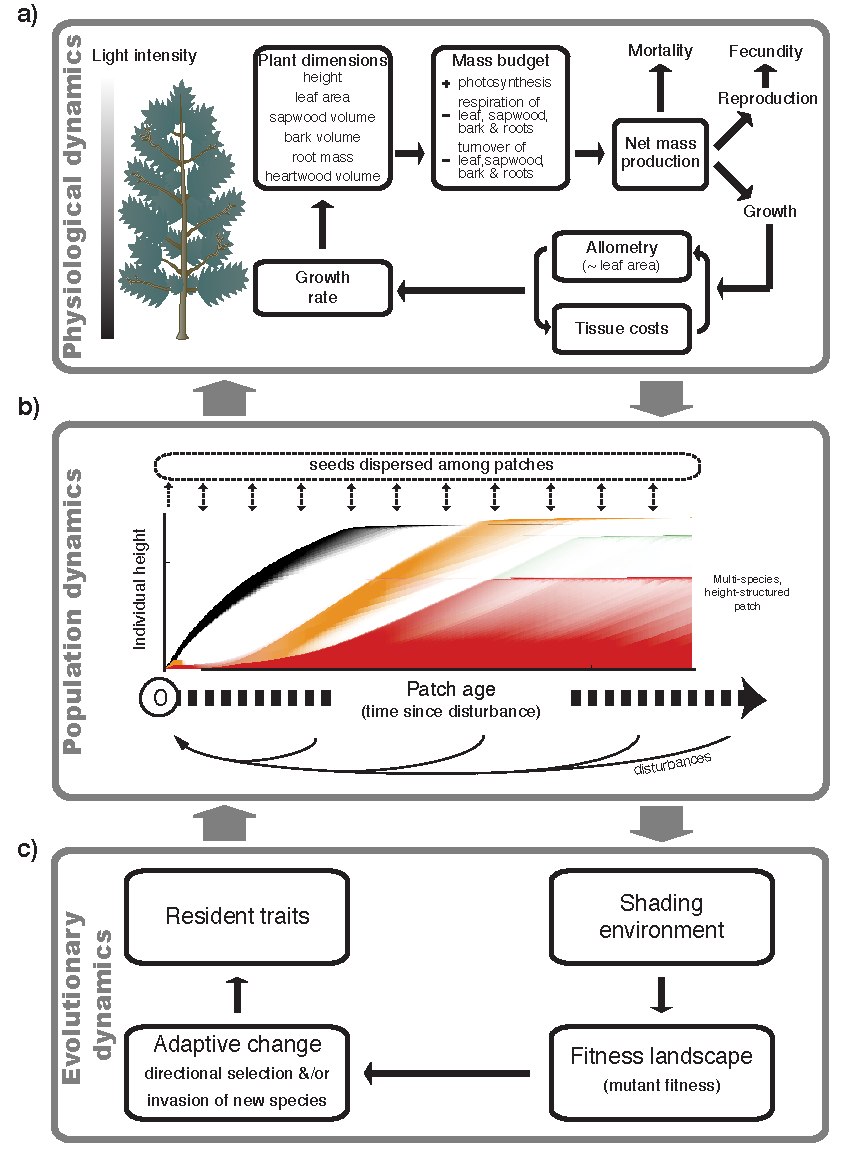
\includegraphics[width=15cm,height=15cm,keepaspectratio]{figures/schematic}

\caption{Processes modelled within {\plant} include physiological, population, and
evolutionary dynamics.
Dynamics across all three levels are driven by the
physiological sub model determining an individual's physiological and
demographic rates on the basis of its traits, size and light environment (a).
(b) Competitive hierarchies  are modelled by tracking the height distribution of
individuals across within a "patch" after a disturbance. The intensity
of shading indicates the density of individuals at a given height for
different species (distinguished by colours). A size- and patch-structured
metapopulation consists of a distribution of patches linked by seed dispersal.
Disturbances occasionally remove all vegetation within a patch, resetting the
patch. (c) The traits of the resident species determine the shading environment
across the metapopulation, which in turn determines the fitness landscape.
Resident traits adjust through directional selection up the fitness landscape
and through the introduction of new species. Adapted from
\citet{Falster-2011}, \citet{Falster-2015}. }

\label{fig:schematic}
\end{figure}

\newpage

\begin{figure}[h!]
\centering
\includegraphics[width=15cm,height=15cm,keepaspectratio]{figures/plant.pdf}
\caption{Physiological dynamics for individual plants vary with size, trait
and light environment. (a) Growth trajectories for plants differing in light
environment and trait (LMA, low = 0.1, solid line; high =  0.267, dashed
line). Lower light environments slow trajectories and interact non-linearly
with traits. (b) Over time, the fraction of living tissue switches from leaf
towards sapwood, with high LMA species having relatively more mass in leaf
than low LMA species. (c) Growth rates peak around 5m high, but this position
varies with both trait and light level (note that this is the derivative of
panel (a)). (d) Growth rates vary with plant size (seedling and mature shown)
and with traits; growth rate differences are more pronounced in high light.
Whole plant light compensation points emerge from the model as the point where
growth rate is zero (x intercept).  The light level used in panels (a) and (c)
is indicated with dots.  See Appendix \ref{sec:plant} for details and code.}
% TODO[Note from James]: [Could you put delta symbols on the y axis rather than d? Also there is alot going in these figures with 4 lines each. You could make it easier for the reader by adding the dashed lines to the keys]
\label{fig:plant}
\end{figure}

\newpage

\begin{figure}[h!]
\centering
\includegraphics[width=15cm,height=15cm,keepaspectratio]{figures/patch.pdf}
\caption{Population dynamics for two species competing within a patch. Lines
in panels (a) same growth trajectories for individuals on the
boundary of successive "cohorts" for each species, using a schedule of 
introduction times generated by an adaptive refinement algorithm.
 Red lines are the low LMA
species from figure \ref{fig:plant}, blue lines are the high LMA species.  The
initial growth rate advantage of the low LMA species (see Figure
\ref{fig:plant} c) means it quickly over tops the high LMA species,
suppressing its growth.  Self-thinning leaves space for the high LMA species
to establish below the canopy of the fast species. Panel (b) shows the same
trajectories as in panel (a), but with shading indicating the density $n$ of
individuals at given size and patch age (light = low density, dark = high density).  
(c) The leaf area index at ground
level for each species.  The dotted line is the total leaf area index (sum
across both species). See Appendix \ref{sec:patch} for details and code.}
\label{fig:patch}
\end{figure}

\newpage

\begin{figure}[h!]
\centering
\includegraphics[width=15cm,height=15cm,keepaspectratio]{figures/emergent.pdf}
\caption{Emergent size-distributions across a metapopulation.
Grey lines show patterns within individual patches differing in time
since disturbance (age), with blue lines indicating patches of a
specific age. Panels show (a) patterns of abundance, (b) leaf area and
(c) height growth rate against size. Note that units of panels (a) and
(b) are per unit height and per unit ground area, respectively.  See Appendix \ref{sec:emergent} for details and code.}
\label{fig:emergent}
\end{figure}

\newpage

\begin{figure}[h!]
\centering
\includegraphics[width=15cm,height=15cm,keepaspectratio]{figures/fitness.pdf}
\caption{Example fitness landscape for LMA, showing potential for stable
coexistence of multiple types.  Fitness is the log of the population growth
rate - at zero species are at equilibrium, above zero they will increase in
density.  (a) Landscape generated by a single species.  At LMA of 0.1 (the
dashed line) there is directional selection for smaller LMA.  At LMA of 0.08
(solid line) there is a branching point (see inset for more detail).  (b)
Landscape generated by two species, holing the first at LMA of 0.08.
Introducing a species at the maximum fitness value from panel (a) reduces the
region of positive fitness considerably (dashed line).  Dotted lines show
subsequent invasions and replacements of the second species, and the solid
line shows a stable fitness landscape where both species exist on a peak in
the fitness landscape.  At this point no further invasion is
possible.  See Appendix \ref{sec:fitness} for details and code.}
\label{fig:fitness}
\end{figure}

\clearpage
\setcounter{secnumdepth}{1}

\begin{appendices}\label{sec:appendices}

\section{Default physiological model for {\plant}}\label{sec:FFW16}

See attached file \url{vignette_physiology.pdf}

\section{Modelling demography in the {\plant} package}\label{sec:demography}

See attached file \url{vignette_demography.pdf}

\section{Plant level properties}\label{sec:plant}

See attached file \url{vignette_plant.R}

\section{Cohort spacing}\label{sec:cohort-spacing}

See attached file \url{vignette_cohort_spacing.R}

\section{Solving for equilibrium seed rain}\label{sec:equilibrium}

See attached file \url{vignette_equilibrium.R}

\section{Patch level dynamics}\label{sec:patch}

See attached file \url{vignette_patch.R}

\section{Patch level emergent properties}\label{sec:emergent}

See attached file \url{vignette_emergent.R}

\section{Calculating fitness in the {\plant}  package}\label{sec:fitness}

See attached file \url{vignette_fitness.R}

\section{Modifying parameters of physiological model}\label{sec:parameters}

See attached file \url{vignette_parameters.R}

\end{appendices}
\end{document}
